\chapter{Description of the apparatus}
\section{General overview}
The setup we used featured the typical photoacoustic experiment characteristics. There was a source of light, a laser in our case, impinging on the gas into a cavity. A mechanical chopper provided a modulation of the light in order to match a proper frequency of the cavity. The acoustic signal, detected by microphones, was filtered by a lock-in amplifier referenced with the chopping frequency. The light path was controlled trough optical elements such as mirrors, lenses and beam-splitters. 
\begin{figure}[!bhpt]\centering
\includegraphics[width=\linewidth, draft=\foto]{eps/laser_diagram.eps}
\caption{Diagram of the experimental apparatus.}
\label{diagram}
\end{figure}

The laboratory instrumentation shown in \cref{instrument} was used to take measurements and drive the various devices.
\begin{figure}[t]\centering
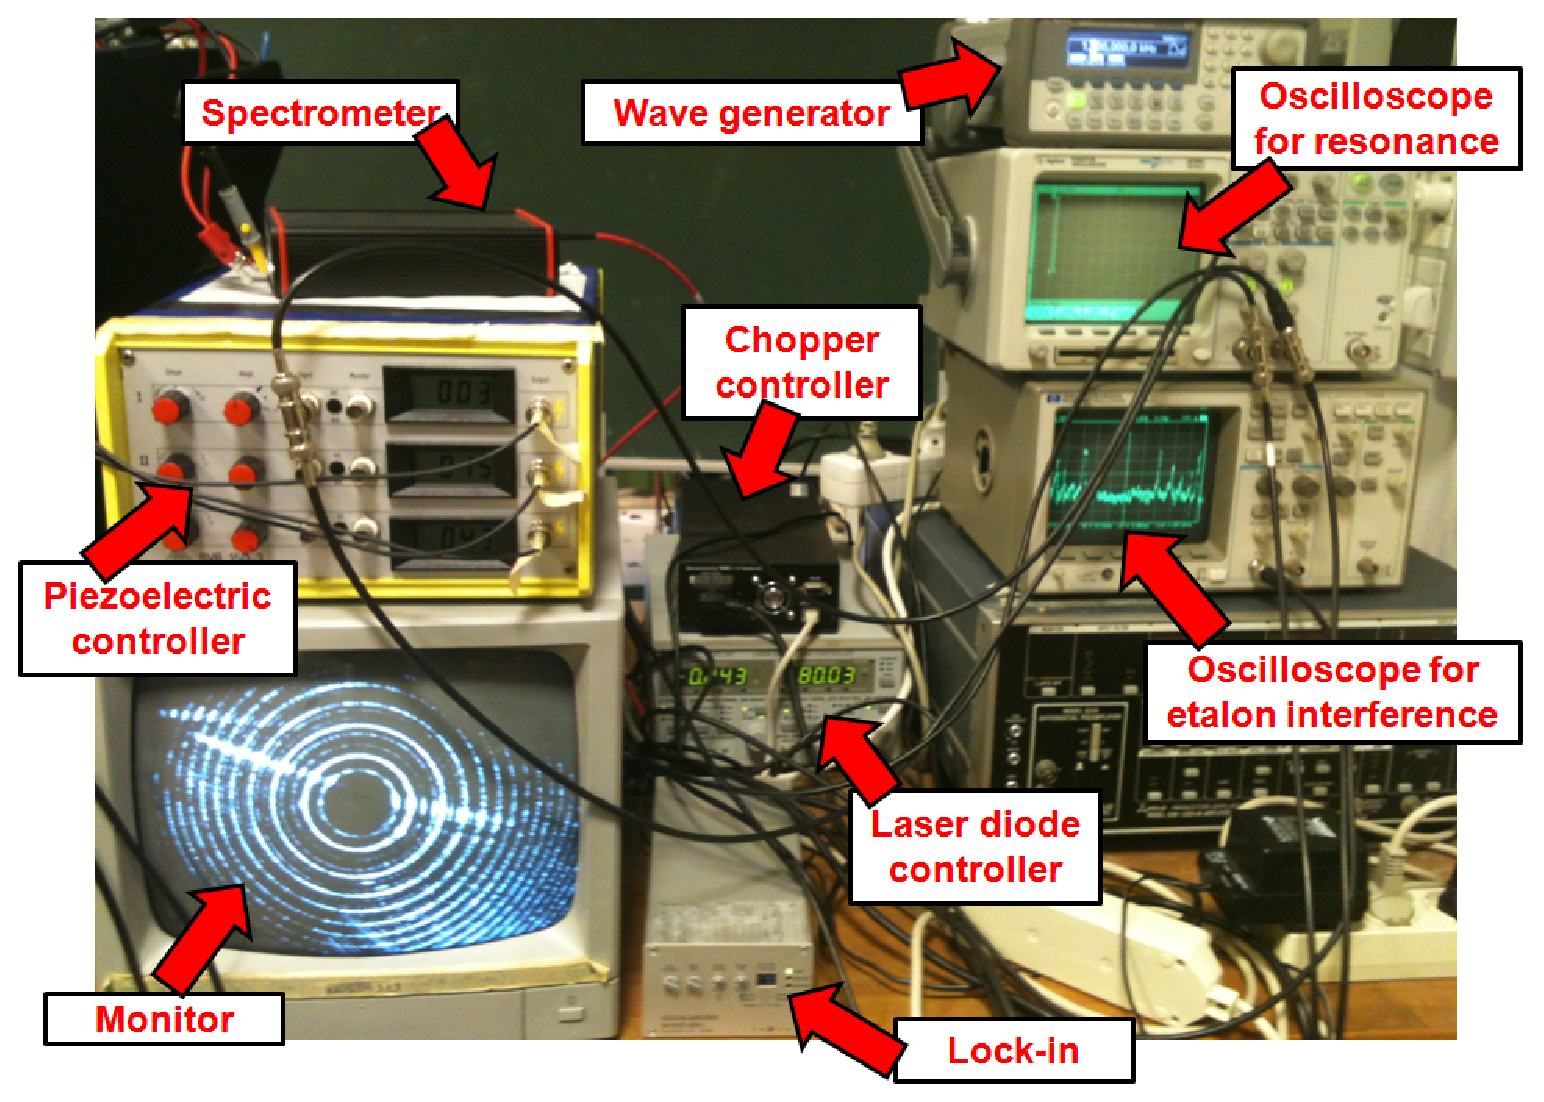
\includegraphics[width=\linewidth, draft=\foto]{eps/instrument.eps}
\caption{Electronic instrumentation used to control the apparatus.}
\label{instrument}
\end{figure}
Other elements we used include:
\begin{itemize}
\item $\pm$15 V power supplier for the microphones
\item membrane vacuum pump
\item rubber pipes and valves to control the gas flow.
\end{itemize}
The data series were acquired with a computer, via a dynamic signal acquisition module\footnote{National Instrument PCI-4462: \url{http://www.ni.com/pdf/manuals/373770j.pdf}}, running the following software:
\begin{itemize}
\item \textit{Avasoft}\textsuperscript{\copyright} by Avantes, the software provided along with the Avaspec spectroscope
\item \textit{Signal Express}\textsuperscript{\texttrademark} by labVIEW\textsuperscript{\texttrademark}
\item \textit{Spectrum}, a labVIEW\textsuperscript{\texttrademark} virtual instrument installed on the laboratory PCs.
\end{itemize}
 We shall now describe in more details the core elements of the apparatus.
\section{The laser source}\label{lasersource}
We used an external cavity laser device, formed by the following elements:
\begin{itemize}
\item a single mode multi-quantum well \ce{AlGaInP}
 laser diode\footnote{Hitachi HL6738MG: \url{http://pdf.datasheetcatalog.com/datasheets/50/502031_DS.pdf}}.
 The lasing wavelength could be tuned from about 680 nm to 695 nm by adjusting the driving current and the diode temperature.
\item a temperature controller case\footnote{Thorlabs TCLDM9: \url{http://www.thorlabs.de/Thorcat/1900/TCLDM9-Manual.pdf}} to set the temperature of the diode. 
\item an external cavity, i.e. a setup that feeds back the laser diode with the first diffraction order of a 1800 grooves/mm grating. Namely, we implemented the so called Littrow configuration (\cref{Littrowsection}). The external cavity allowed us to better select a given lasing mode, thus getting a smaller emission linewidth. The grating was put on a piezoelectric mechanical actuator\footnote{Thorlabs KC1-T-PZ/M: \url{http://www.thorlabs.de/Thorcat/2400/KC1-T-PZ_M-AutoCADPDF.pdf }}, which permitted nm-order adjustments of its position. Since a grating diffracts different frequencies at different angles, moving the grating we could control the frequency fed back to the laser and thus enhanced. This is how we got a fine tuning of the frequency, and how we were able to make the 2-3 GHz scan to see the absorption line (more on this in \cref{tuna}).
\end{itemize} 
\section{The acoustic chamber} 
 The gas to analyze, pure \ce{O2} at atmospheric pressure, was contained in a brass chamber, featuring :
\begin{itemize}
	\item an internal cavity, about \mbox{10 cm} long, where the gas actually resonated. Other two smaller cavities, half as long, were present before and after the main cavity. Since we couldn't open the brass chamber, we had no way to accurately measure the dimensions and the position of the main cavity with respect to the other two ones. It should be noticed that our chamber had been recycled from another experiment and was not explicitly thought for the usage we do of it
	\item four microphones put about halfway in the chamber, one for each side of it. Due to the fact that the chamber couldn't be opened, we don't know whether the microphones were actually halfway. Anyway a possible misplacement would not affect the validity of our measurement, as it would result just in a less intense signal
	\item an active strain gauge vacuometer\footnote{Edwards ASG-1000-NW16:\vspace{-10pt}\begin{flushright}\url{http://www.ultimatevacuum.dk/D35725880\%20ASG\%20user\%20manual.pdf }\end{flushright}} to measure the pressure in the chamber. 
\end{itemize}

\section{Reference arm}\label{referencearm}
Once generated in the ECDL, the laser beam was split by a simple glass into two rays: one going through the chopper and entering the acoustic chamber, the other passing  through an etalon. The interference pattern (see \cref{etalon}) was monitored with a video camera. This was useful, since the the spectroscope resolution, as reported in \cref{shapeaks}, was too poor to detect the small laser frequency shifts due to fine tuning with the external cavity. The etalon instead could detect this shift as a variation of the diameter in the diffraction rings. Moreover, the PAL analogic video signal could be observed with an oscilloscope as well, to get a quantitative measurement of the rings movements thanks to the measurement functions of the instrument. The etalon allowed also to detect a multimodal emission much more immediately than the spectroscope.